\chapter{State of the Art}
\label{chap:sota}

\section{Introduction}

This chapter reviews the technical background needed to understand the rest of the report. It covers the \gls{can} bus and the protocols built on top of it, the main attack classes documented against it, existing intrusion detection approaches, and how machine learning has been applied to this specific problem. The chapter ends with a comparison of existing approaches and a statement of the research gap this project addresses.

\section{Electric vehicles and in-vehicle networks}

An electric vehicle replaces the internal combustion drivetrain with a battery pack, one or more electric motors, and a battery management system, but it keeps the same general electrical architecture as a combustion vehicle: dozens of \gls{ecu}s, each responsible for one function (battery management, motor control, braking, infotainment, driver assistance), connected by one or more internal networks. Electric vehicles typically add safety-critical, high-frequency messages related to battery state, state of charge, and motor torque, which increases the number of messages an intrusion detection system has to understand correctly.

Because manufacturers rarely publish the internal message layout of their vehicles, most of the practical knowledge about a specific vehicle's \gls{can} traffic comes from reverse-engineered \gls{dbc} files produced by the community, from UDS diagnostic responses, or from vendor tools. This project relies on both sources, as described in Chapter~\ref{chap:design}.

\section{The CAN bus}

\subsection{Overview}

The Controller Area Network (\gls{can}) is a broadcast serial bus standardized by ISO~11898~\cite{iso11898}. Every \gls{ecu} on the bus can transmit and receive; there is no central master. Each message (frame) carries an identifier and up to 8 bytes of payload in classic \gls{can}. The identifier does not name a sender or a receiver — it names the \emph{content} of the message, and every node decides for itself whether a given identifier is relevant to it.

\begin{figure}[H]
\centering
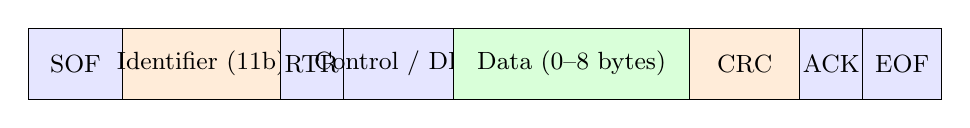
\begin{tikzpicture}[font=\small, scale=1.0]
\def\h{0.9}
\draw[fill=blue!10] (0,0) rectangle (1.2,\h) node[midway]{SOF};
\draw[fill=orange!15] (1.2,0) rectangle (3.2,\h) node[midway]{Identifier (11b)};
\draw[fill=blue!10] (3.2,0) rectangle (4.0,\h) node[midway]{RTR};
\draw[fill=blue!10] (4.0,0) rectangle (5.4,\h) node[midway]{Control / DLC};
\draw[fill=green!15] (5.4,0) rectangle (8.4,\h) node[midway]{Data (0--8 bytes)};
\draw[fill=orange!15] (8.4,0) rectangle (9.8,\h) node[midway]{CRC};
\draw[fill=blue!10] (9.8,0) rectangle (10.6,\h) node[midway]{ACK};
\draw[fill=blue!10] (10.6,0) rectangle (11.6,\h) node[midway]{EOF};
\end{tikzpicture}
\caption{Simplified structure of a classic CAN data frame (11-bit identifier).}
\label{fig:can-frame}
\end{figure}

Figure~\ref{fig:can-frame} shows the simplified layout of a classic \gls{can} data frame. The identifier also sets the message priority: during arbitration, the frame with the numerically lowest identifier wins the bus, so low identifiers are generally reserved for the most safety-critical messages. This project's replay engine reconstructs exactly these three fields — timestamp, identifier, and payload bytes — from every supported log format, as described in Section~\ref{sec:impl-parser}.

\subsection{CAN FD}

\gls{canfd} extends classic \gls{can} with two changes: the data payload can go up to 64 bytes instead of 8, and the data phase of the frame can run at a higher bit rate than the arbitration phase. \gls{canfd} is increasingly used on newer vehicle platforms, including some of the electric vehicles used in this project's training corpus (Chapter~\ref{chap:validation}), where a single \gls{canfd} frame can carry several sensor readings that would otherwise need multiple classic \gls{can} frames.

\subsection{UDS}

\gls{uds}, standardized as ISO~14229~\cite{iso14229}, defines a request/response diagnostic protocol running on top of \gls{can}. A diagnostic tool sends a service request (for example \texttt{0x22 ReadDataByIdentifier} or \texttt{0x10 DiagnosticSessionControl}) to a specific \gls{ecu} address, and the \gls{ecu} replies with the requested data or an error code. Several datasets used in this project (Chapter~\ref{chap:validation}) were captured by polling a vehicle's \gls{ecu}s with \gls{uds} requests rather than by passively recording broadcast traffic, which changes the expected traffic pattern: request/response pairs at a fixed polling interval, instead of continuously broadcast sensor frames.

\subsection{ISO-TP}

Because a classic \gls{can} frame only carries 8 payload bytes, \gls{uds} responses longer than that must be split across several frames. \gls{isotp}, standardized as ISO~15765-2~\cite{iso15765}, defines how this segmentation works: a First Frame announces the total message length, and one or more Consecutive Frames carry the remaining bytes, each with a sequence number. A decoder that only understands single-frame \gls{can} payloads will misinterpret a multi-frame \gls{isotp} response as several unrelated short frames.

\subsection{OBD-II}

\gls{obd} (SAE~J1979~\cite{sae_j1979}) is a standardized subset of vehicle diagnostics, accessible through a physical connector present in virtually every vehicle sold after the mid-2000s. It defines standard parameter identifiers (PIDs) for common values such as vehicle speed or engine coolant temperature. \gls{obd} adapters, including low-cost ELM327 devices, are one of the most common ways to get \gls{can} bus access to a vehicle without opening the dashboard, and are the entry point supported by this project's live hardware capture mode (Chapter~\ref{chap:design}).

\section{Known CAN bus attacks}

The \gls{can} bus has no authentication, no encryption, and no reliable way to identify the sender of a frame. This has been demonstrated repeatedly in the security literature. Koscher~et al.~\cite{koscher2010experimental} showed that an attacker with physical access to a vehicle's internal network could manipulate safety-critical functions by simply injecting crafted \gls{can} frames. Miller and Valasek~\cite{miller2015remote} later demonstrated a remote version of this attack, controlling a production vehicle's steering and braking over its cellular connection without any physical access at the time of the attack. These two results are widely cited as the moment automotive cybersecurity became a mainstream concern rather than a theoretical one.

From an intrusion-detection point of view, published attacks and public datasets group into a small number of recurring patterns, all of which this project's detection pipeline is designed to catch:

\begin{itemize}
    \item \textbf{Denial-of-service / flooding.} The attacker transmits a high-priority identifier (often \texttt{0x000}) at a very high rate, starving the bus and preventing legitimate frames from being transmitted.
    \item \textbf{Fuzzing.} The attacker transmits frames with random or semi-random identifiers and payloads, looking for an \gls{ecu} that reacts unexpectedly.
    \item \textbf{Spoofing / injection.} The attacker transmits frames with a legitimate identifier but a forged payload, for example to report a false speed or gear state.
    \item \textbf{Replay.} The attacker records legitimate traffic and re-transmits it later, out of its original context, to re-trigger a past command.
    \item \textbf{Masquerade.} A refinement of injection in which the attacker first suppresses the legitimate sender of an identifier, then injects forged frames on the same identifier at the expected rate, so that simple frequency-based detectors do not notice anything unusual. This pattern is explicitly represented in the ROAD dataset~\cite{verma2020road}, which distinguishes plain injection attacks from their masqueraded counterparts.
\end{itemize}

\section{Intrusion detection systems for CAN}

Intrusion detection approaches for the \gls{can} bus are usually grouped into three families.

\textbf{Signature-based detection} matches observed traffic against a database of known attack patterns. It is precise for known attacks but cannot detect a new attack it has not seen before, and \gls{can} traffic rarely carries enough structure (no protocol fields beyond identifier and payload) to write rich signatures.

\textbf{Specification-based detection} encodes expected behaviour by hand: expected identifiers, expected frequency ranges, expected payload ranges. It is transparent and does not need attack data to train, but it needs a specification for every vehicle and message, and it does not generalize to unexpected but legitimate variations in traffic.

\textbf{Anomaly-based detection} learns what normal traffic looks like (from timing, payload statistics, or both) and flags deviations. This is the approach with the widest applicability across vehicles, because it does not need an attack signature or a hand-written specification, only a sample of normal traffic. It is also the family this project belongs to, combined with a persistence layer to reduce single-frame false positives.

\section{Machine learning for CAN intrusion detection}

Because \gls{can} frames are small, frequent, and mostly periodic, unsupervised anomaly detection is a natural fit: normal traffic is abundant, while labelled attack traffic is comparatively rare and vehicle-specific. Two techniques are particularly relevant to this project.

\textbf{Isolation Forest}~\cite{liu2008isolation} builds an ensemble of random decision trees that isolate each data point by repeated random splits. Points that are easy to isolate (short average path length across the trees) are scored as more anomalous than points that need many splits to separate from the rest of the data. It does not require labelled attack data, its per-sample cost is low, and it does not assume a particular data distribution, which makes it a common choice for this problem. It is the model used by this project's per-vehicle scoring layer (Chapter~\ref{chap:design}).

\textbf{K-Means clustering}~\cite{macqueen1967methods} partitions data into a fixed number of clusters by minimizing the distance between each point and its cluster centroid. In this project it is used not to detect anomalies directly, but to classify the vehicle's current operating state (parking, idle, driving) from timing and payload features, so that the correct per-state Isolation Forest model can be selected. Chapter~\ref{chap:validation} documents a defect found in this exact classification step and how it was diagnosed and corrected.

Beyond classical models, GAN-based intrusion detection has also been explored in the literature: Seo~et al.~\cite{seo2018gids} proposed GIDS (GAN-based Intrusion Detection System), trained and evaluated on the Car-Hacking dataset, one of the most widely used public benchmarks for \gls{can} \gls{ids} research together with the ROAD dataset~\cite{verma2020road} used in this project's own training corpus (Chapter~\ref{chap:validation}).

\section{Related work and comparison}

Table~\ref{tab:sota-comparison} compares the main families of approaches discussed above against the design adopted in CANvisionNative.

\begin{table}[H]
\centering
\caption{Comparison of CAN IDS approaches.}
\label{tab:sota-comparison}
\begin{tabularx}{\textwidth}{@{}lXXXX@{}}
\toprule
\textbf{Approach} & \textbf{Detects unknown attacks} & \textbf{Vehicle-specific} & \textbf{Needs attack data} & \textbf{Human-readable output} \\
\midrule
Signature-based & No & Depends on DB & Yes & No \\
Specification-based & Partially & Yes (by hand) & No & No \\
Single statistical (timing or payload only) & Partially & No & No & No \\
Single-model ML (e.g.\ one Isolation Forest for all vehicles) & Yes & No & No & No \\
GAN-based (e.g.\ GIDS~\cite{seo2018gids}) & Yes & Depends on training set & No & No \\
\textbf{CANvisionNative (this project)} & \textbf{Yes} & \textbf{Yes (per-vehicle model)} & \textbf{No} & \textbf{Yes (rule-based + LLM)} \\
\bottomrule
\end{tabularx}
\end{table}

Most published anomaly-based approaches evaluate a single detection signal (usually either timing or a single ML model) against a single dataset, and report a numeric score without producing a human-readable explanation of the anomaly. Vehicle-specific model selection, when discussed at all, is usually treated as future work rather than an implemented feature.

\section{Research gap}

From this review, three gaps stand out that motivated the design choices of this project:

\begin{enumerate}
    \item Most anomaly-based \gls{can} \gls{ids} designs in the literature rely on a single detection signal. Combining independent signals (timing, payload, machine learning, temporal persistence) into one fusion score, so that an attack missed by one layer can still be caught by another, is comparatively rare outside research prototypes.
    \item Vehicle-specific behaviour is well documented as a challenge, but concrete systems that select a per-vehicle trained model at run time, rather than a single generic model, are uncommon in practice — and, as Chapter~\ref{chap:validation} shows, easy to get wrong silently even when the code appears to support it.
    \item Explaining a detected anomaly in plain language, rather than presenting a raw numeric score, is largely absent from the reviewed anomaly-detection literature, which focuses on detection accuracy rather than analyst usability.
\end{enumerate}

CANvisionNative addresses these three gaps directly: a four-layer fusion score (Chapter~\ref{chap:design}), a per-vehicle model store selected at run time (Chapter~\ref{chap:design} and Chapter~\ref{chap:impl}), and a rule-based plus \gls{llm} explanation pipeline (Chapter~\ref{chap:design}).

\section{Conclusion}

This chapter presented the \gls{can} bus and its related protocols, the main documented attack classes, and the three families of intrusion detection approaches, with particular attention to how machine learning has been applied to this problem. The comparison in Table~\ref{tab:sota-comparison} positioned this project's four-layer, vehicle-specific, explainable design against existing approaches. The next chapter turns this context into a concrete requirements analysis for CANvisionNative.
